\section{Rarefied gas flows}

\subsection{The Knudsen number}
For gases we define their \textit{Mean Free Path} as the average distance that 
the molecules of this gas are travelling without taking part in collisions.
The MFP of a hard-sphere gas in thermodynamic equilibrium is given by the equation~\cite{Zhang2012}:
\begin{equation}
 \lambda = \frac{1}{\sqrt{2} \pi \cdot n_\mathrm{g} \cdot d^2}
 \label{eq:MFP}
\end{equation}
where $d$ is the mean molecular diameter and $n_\mathrm{g}$ the number density of the gas.
Referring to the mean molecular spacing as $\delta$, $n_\mathrm{g}=\delta^{-3}$.
For air at atmospheric conditions ($T=298\,\mathrm{K}$, $p=1\,\mathrm{atm}$),
$\lambda_{\mathrm{air}} = 6.111\cdot10^{-8}\,\mathrm{m}$
while for the (lighter and smaller) helium 
$\lambda_{\mathrm{He}} = 17.651\cdot10^{-8}\,\mathrm{m}$.~\cite{Karniadakis_Microflows}

Knowing the MFP of a gas we can compute the \textit{Knudsen number} for a given scale.
This is defined as the ratio of the MFP to the characteristic length $L_0$ of the geometry:
\begin{equation}
 \mathrm{Kn} := \frac{\lambda}{L_0}
 \label{eq:Kn_def}
\end{equation}
The length $L_0$ can also be a limit above which very large variations of a macroscopic
quantity $\Phi_0$ may be observed and we can also write:
\begin{equation}
 \mathrm{Kn} \approx \frac{\lambda}{\Phi_0} \cdot \Big|\frac{\mathrm{d}\Phi_0}{\mathrm{d}L_0}\Big|
 \label{eq:Kn_phi}
\end{equation}
In complex geometries, a local Knudsen number can be chosen to solve the problem
of deciding about the characteristic length.
Equation~\ref{eq:Kn_phi} gives a good intuition for the relevance of the Knudsen number with
the continuity assumption, as in ``continuous'' scenarios (small $\mathrm{Kn}$) we would expect small
variations of macroscopic quantities. We can also relate the
Knudsen number to the Mach and Reynolds numbers~\cite{Zhang2012}:
\begin{equation}
 \mathrm{Kn} = \frac{\lambda}{L_0} \cdot \sqrt{\frac{\pi \gamma}{2}} \cdot \frac{\mathrm{Ma}}{\mathrm{Re}}
 \label{eq:Kn_Ma}
\end{equation}
where $\gamma := c_p / c_V$ is the specific heat capacity ratio of the gas.



\subsection{Division of the gas flow regimes}
The Knudsen number can be used to divide different \textit{flow regimes} and a
rough, empirical classification can be found in figure~\ref{fig:flow_regimes}.~\cite{Zhang2012} 
The region $\mathrm{Kn}<10^{-2}$ (or $\mathrm{Kn}<10^{-3}$, as more recently suggested)
is referred to as the \textit{continuum regime}, in which the thermodynamic equilibrium
assumptions hold and the application of the Navier-Stokes equations with the usual
no-slip boundary conditions is valid.
The other part of the range, where $\mathrm{Kn}>10$, corresponds to the
\textit{free molecular regime}. In this area, the molecules almost do not collide
with each other.

In between, the gas flow may belong to the \textit{slip-flow regime}
($10^{-2} < \mathrm{Kn} < 10^{-1} $) or to the \textit{transition regime}
($10^{-1} < \mathrm{Kn} < 10 $). In the slip-flow regime, methods assuming 
continuity can still be applied but they will fail near the walls, as there
non-equilibrium effects like temperature jump dominate and the no-slip condition
cannot be satisfied. In the transition regime, the thermodynamic equilibrium
assumptions begin to break down, as the ``Knudsen layer'' forces
a non-linear stress-strain relationship for the flow near the wall.

Which regimes are mainly of practical interest? The term \textit{Rarefied Gas Flows} 
usually refers to the slip-flow and the
transition regime. As an example, $\mathrm{Kn}=1$ for air 
is achieved around length scale $L_0 = 65\,\mathrm{nm}$.
In some applications, different scales and flow regimes may be paired (\textit{mixed flow regimes}),
leading in the need to study transport phenomena in a wide Knudsen range.~\cite{Karniadakis_Microflows}

\begin{figure}[h!]%
 	\begin{center}%
 		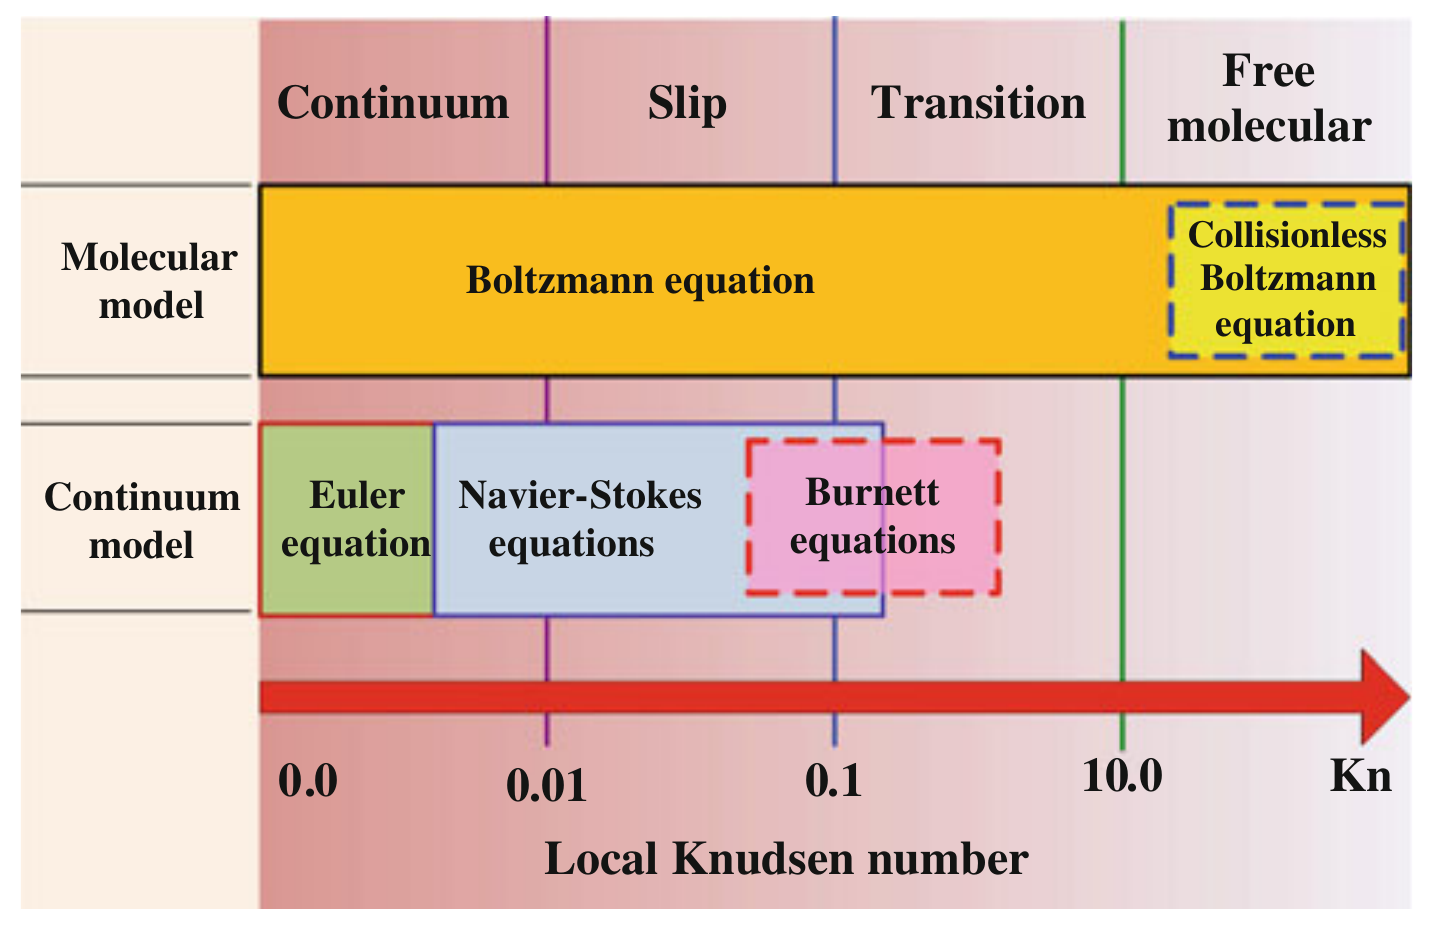
\includegraphics[scale=0.2]{flow_regimes}%
 		\caption{Division of the gas flow regimes in relation to the Knudsen 
 		number, along with the limits of different CFD 
 		approaches.~\cite{Zhang2012}}\label{fig:flow_regimes}%
 	\end{center}%
\end{figure}